\documentclass[12pt,a4paper]{article}
\usepackage[utf8]{inputenc}
\usepackage[portuguese]{babel}
\usepackage{graphicx}
\usepackage{float}
\usepackage{amsmath}
\usepackage{geometry}
\usepackage{hyperref}
\usepackage{caption}

\geometry{margin=2.5cm}

% Capa
\title{
    \Large\textbf{Universidade de Fortaleza - UNIFOR}\\
    \large Curso de Ciência da Computação\\
    \vspace{1.5cm}
    \huge\textbf{Análise de Rede de Colaboração Científica}\\
    \large General Relativity and Quantum Cosmology (ca-GrQc)
}
\author{João Pedro Brasil}
\date{12 de fevereiro de 2026}

\begin{document}

\maketitle
\thispagestyle{empty}
\newpage

\tableofcontents
\newpage

\section{Introdução}

Este relatório apresenta uma análise estrutural da rede de colaboração científica na área de Relatividade Geral e Cosmologia Quântica (General Relativity and Quantum Cosmology), disponibilizada publicamente pelo Stanford Network Analysis Project (SNAP) \cite{snapnets}.

\subsection{Descrição do Dataset}

O dataset \textit{ca-GrQc} representa uma rede de colaboração entre pesquisadores, onde:

\begin{itemize}
    \item \textbf{Vértices}: Representam autores individuais de artigos científicos
    \item \textbf{Arestas}: Representam colaborações entre dois autores (co-autoria em artigos)
    \item \textbf{Fonte}: arXiv - repositório de preprints científicos
    \item \textbf{Período}: Artigos submetidos até abril de 2003
    \item \textbf{URL}: \url{https://snap.stanford.edu/data/ca-GrQc.html}
\end{itemize}

Este tipo de rede é classificado como uma \textbf{rede social não-direcionada}, onde as conexões são simétricas (se A colabora com B, então B colabora com A).

\subsection{Objetivos da Análise}

Os principais objetivos deste trabalho são:

\begin{enumerate}
    \item Caracterizar a estrutura topológica da rede de colaboração
    \item Calcular métricas fundamentais de teoria dos grafos
    \item Analisar a distribuição de graus dos vértices
    \item Visualizar a estrutura da rede
    \item Interpretar os resultados no contexto da colaboração científica
\end{enumerate}

\section{Metodologia}

A análise foi realizada utilizando Python 3.12, com as seguintes bibliotecas:

\begin{itemize}
    \item \texttt{networkx}: Manipulação e análise de grafos
    \item \texttt{matplotlib}: Visualização de dados
    \item Implementação personalizada da estrutura de grafo
\end{itemize}

As métricas calculadas incluem:
\begin{itemize}
    \item Ordem do grafo (número de vértices)
    \item Tamanho do grafo (número de arestas)
    \item Densidade do grafo
    \item Grau mínimo e máximo
    \item Distribuição de graus
\end{itemize}

\section{Resultados}

\subsection{Métricas Estruturais}


A análise da rede revelou as seguintes características estruturais:

\begin{table}[H]
\centering
\caption{Métricas principais da rede ca-GrQc}
\begin{tabular}{|l|r|}
\hline
\textbf{Métrica} & \textbf{Valor} \\
\hline
Ordem (Vértices) & 5.242 \\
Tamanho (Arestas) & 28.980 \\
Densidade & 0,0021 \\
Classificação & Esparso \\
Grau Mínimo & 2 \\
Grau Máximo & 162 \\
Grau Médio & $\approx$ 11,06 \\
\hline
\end{tabular}
\end{table}

\subsubsection{Interpretação das Métricas}

\textbf{Densidade:} O valor de densidade de 0,0021 (ou 0,21\%) indica que a rede é \textbf{extremamente esparsa}. Isso significa que apenas uma pequena fração das possíveis conexões entre pesquisadores está presente. A densidade é calculada por:

\begin{equation}
    d = \frac{2E}{V(V-1)} = \frac{2 \times 28.980}{5.242 \times 5.241} = 0,0021
\end{equation}

Este resultado é esperado em redes de colaboração científica, onde cada pesquisador tende a colaborar com um grupo relativamente pequeno de outros pesquisadores.

\textbf{Grau Médio:} O grau médio é calculado como:

\begin{equation}
    \bar{k} = \frac{2E}{V} = \frac{2 \times 28.980}{5.242} \approx 11,06
\end{equation}

Isso indica que, em média, cada pesquisador colabora com aproximadamente 11 outros pesquisadores.

\textbf{Amplitude de Graus:} A diferença significativa entre o grau mínimo (2) e máximo (162) sugere a presença de \textit{hubs} na rede - pesquisadores altamente conectados que colaboram com muitos outros, característica típica de redes \textit{scale-free}.

\subsection{Distribuição de Graus}

A Figura \ref{fig:histogram} apresenta o histograma da distribuição de graus dos vértices na rede.

\begin{figure}[H]
    \centering
    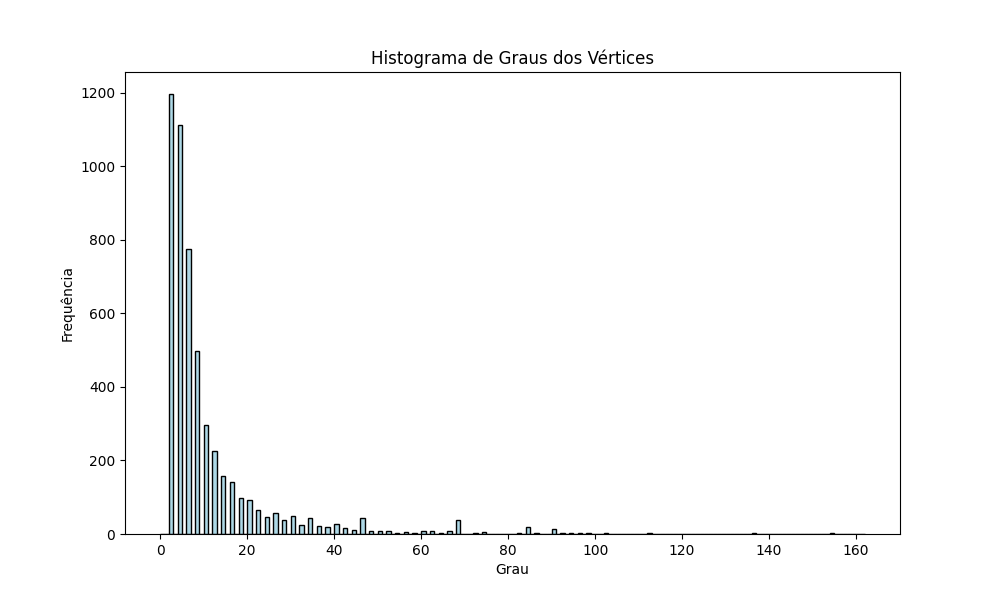
\includegraphics[width=0.85\textwidth]{histogram.png}
    \caption{Histograma da distribuição de graus dos vértices}
    \label{fig:histogram}
\end{figure}

\textbf{Observações sobre a distribuição:}

\begin{itemize}
    \item A distribuição apresenta uma \textbf{cauda longa} (\textit{long tail}), característica de redes \textit{scale-free}
    \item A maioria dos pesquisadores possui baixo número de colaborações (2-20 colaboradores)
    \item Poucos pesquisadores possuem número muito alto de colaborações (acima de 100)
    \item Este padrão sugere uma distribuição de lei de potência, comum em redes sociais e de colaboração
\end{itemize}

Esta distribuição indica que a rede segue o princípio do \textbf{"rich get richer"} (ligação preferencial), onde pesquisadores já bem conectados têm maior probabilidade de estabelecer novas colaborações.

\subsection{Ajuste de Lei de Potência}

Para verificar quantitativamente se a rede segue uma distribuição \textit{scale-free}, foi realizado um ajuste de lei de potência aos dados de distribuição de graus. Uma rede scale-free apresenta uma distribuição de graus que segue a forma:

\begin{equation}
    P(k) \sim k^{-\gamma}
\end{equation}

onde $P(k)$ é a probabilidade de um vértice ter grau $k$, e $\gamma$ é o \textbf{expoente de escala} (ou expoente crítico).

\subsubsection{Resultados do Ajuste}

O ajuste foi realizado utilizando regressão linear no espaço logarítmico ($\log P(k)$ vs. $\log k$). A Figura \ref{fig:power_law} apresenta o gráfico log-log dos dados observados e a curva ajustada.

\begin{figure}[H]
    \centering
    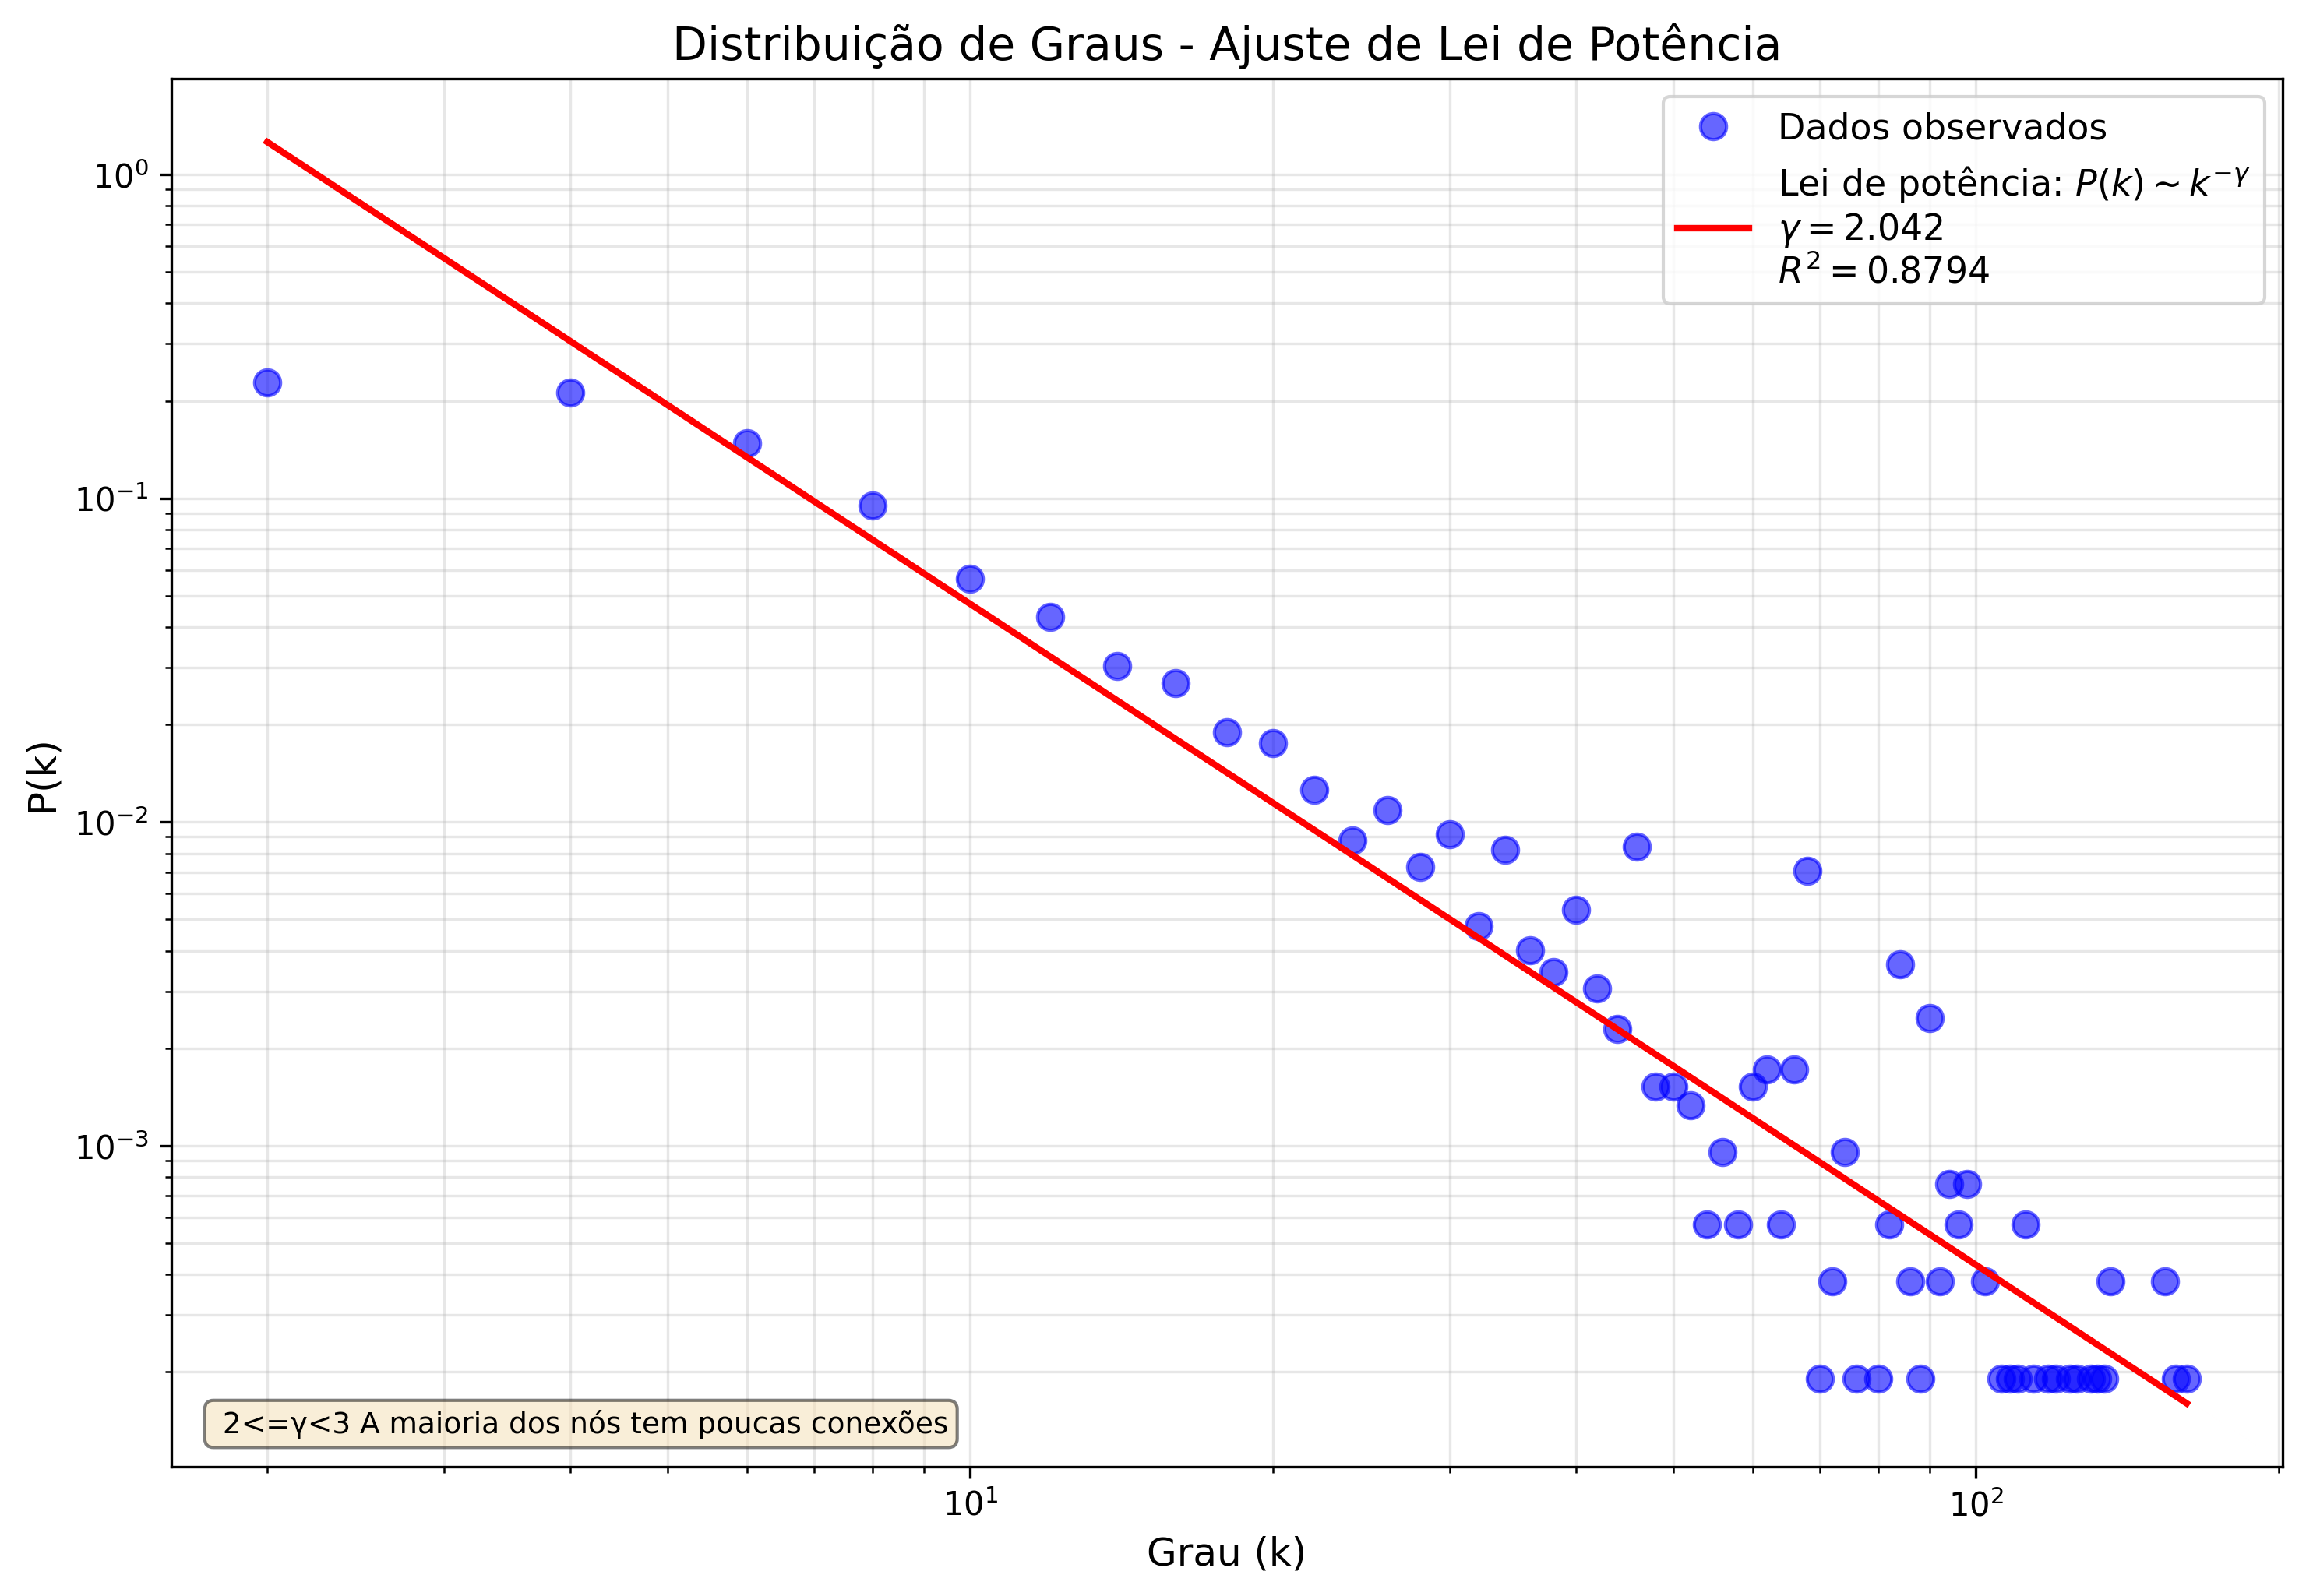
\includegraphics[width=0.9\textwidth]{power_law_fit.png}
    \caption{Ajuste de lei de potência à distribuição de graus em escala log-log. Os pontos azuis representam os dados observados e a linha vermelha o ajuste $P(k) \sim k^{-\gamma}$.}
    \label{fig:power_law}
\end{figure}

Os parâmetros obtidos foram:

\begin{table}[H]
\centering
\caption{Parâmetros do ajuste de lei de potência}
\begin{tabular}{|l|r|}
\hline
\textbf{Parâmetro} & \textbf{Valor} \\
\hline
Expoente $\gamma$ & 2,0416 \\
Coeficiente de determinação ($R^2$) & 0,8794 \\
Grau mínimo considerado ($k_{\text{min}}$) & 2 \\
\hline
\end{tabular}
\end{table}

\subsubsection{Interpretação do Expoente}

O valor do expoente $\gamma = 2,0416$ situa-se no intervalo $2 \leq \gamma < 3$, o que caracteriza uma \textbf{rede scale-free típica}. Este resultado tem importantes implicações:

\begin{enumerate}
    \item \textbf{Média finita, variância infinita}: Neste intervalo, a distribuição possui média bem definida (que corresponde ao grau médio $\approx 11,06$ calculado), mas a variância tende ao infinito no limite termodinâmico. Isso significa que há flutuações muito grandes nos graus dos vértices.
    
    \item \textbf{Presença significativa de hubs}: Valores de $\gamma$ próximos a 2 (chamados de \textit{ultra scale-free}) indicam que a rede possui hubs muito proeminentes. Quanto menor o $\gamma$, mais pronunciada é a presença de vértices altamente conectados.
    
    \item \textbf{Comparação com modelos teóricos}: O modelo de Barabási-Albert, que é o modelo clássico de redes scale-free baseado em ligação preferencial, prevê $\gamma = 3$. O valor observado de $\gamma \approx 2,04$ sugere que a rede ca-GrQc possui um mecanismo de ligação preferencial ainda mais forte que o modelo BA clássico.
    
    \item \textbf{Vulnerabilidade estrutural}: Redes com $\gamma < 3$ são extremamente robustas a falhas aleatórias (remoção de vértices aleatórios), mas muito vulneráveis a ataques direcionados aos hubs. A remoção de poucos pesquisadores altamente conectados poderia fragmentar significativamente a rede.
\end{enumerate}

\subsubsection{Qualidade do Ajuste}

O coeficiente de determinação $R^2 = 0,8794$ fornece um \textbf{indício razoável} de que a rede ca-GrQc segue uma distribuição de lei de potência. Este valor significa que aproximadamente 88\% da variabilidade dos dados é explicada pelo modelo de lei de potência.

A linearidade observada no gráfico log-log (Figura \ref{fig:power_law}) ao longo de quase duas décadas logarítmicas confirma visualmente a natureza scale-free da rede.

\subsubsection{Contexto Científico}

Estes resultados são consistentes com estudos empíricos de redes de colaboração científica:

\begin{itemize}
    \item Newman (2001) \cite{arxiv} encontrou valores de $\gamma$ entre 2,1 e 2,5 para diversas redes de colaboração científica
    \item O fenômeno de ligação preferencial (\textit{preferential attachment}) é bem documentado na ciência: pesquisadores tendem a colaborar com colegas já estabelecidos e bem conectados
    \item A estrutura scale-free facilita a difusão rápida de conhecimento através dos hubs, mas também pode criar desigualdades na visibilidade científica
\end{itemize}

\subsection{Visualização da Rede}

\subsubsection{Visualização Parcial}

A Figura \ref{fig:graph_partial} apresenta uma visualização parcial da rede (primeiros 10 vértices).

\begin{figure}[H]
    \centering
    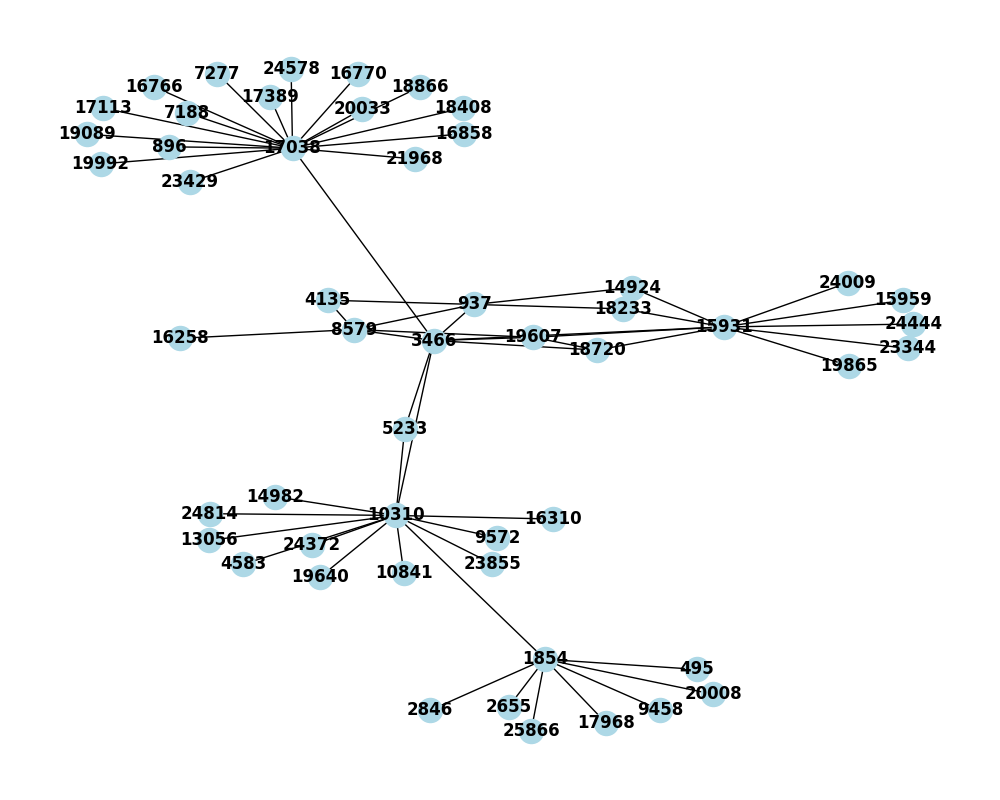
\includegraphics[width=0.85\textwidth]{graph_10.png}
    \caption{Visualização parcial da rede de colaboração (10 primeiros vértices)}
    \label{fig:graph_partial}
\end{figure}

A amostra apresentada ilustra:

\begin{itemize}
    \item Estrutura de conexões entre pesquisadores
    \item Presença de agrupamentos (\textit{clusters})
    \item Diferentes níveis de conectividade entre os nós
\end{itemize}

\subsubsection{Visualização Completa}

A Figura \ref{fig:graph_full} apresenta uma visualização da rede completa com todos os 5.242 vértices.

\begin{figure}[H]
    \centering
    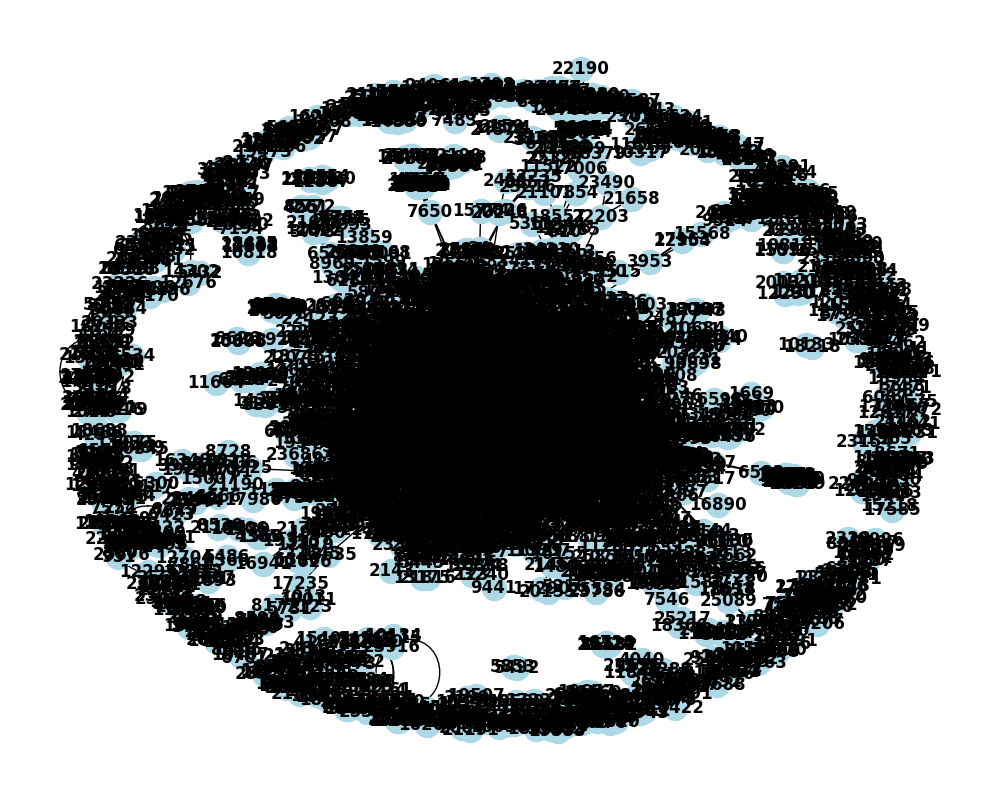
\includegraphics[width=1.0\textwidth]{graph.png}
    \caption{Visualização completa da rede de colaboração científica ca-GrQc. Os nós são coloridos por grau (quanto mais escuro, maior o grau) e seu tamanho é proporcional ao número de colaborações. Observa-se claramente a estrutura \textit{scale-free} com presença de \textit{hubs} altamente conectados.}
    \label{fig:graph_full}
\end{figure}

Apesar da densidade visual, a visualização completa revela importantes características estruturais:

\begin{itemize}
    \item \textbf{Núcleo denso}: Região central altamente conectada com os pesquisadores mais prolíficos
    \item \textbf{Periferia esparsa}: Grupos de pesquisadores com poucas colaborações nas bordas
    \item \textbf{Hubs visíveis}: Nós de maior tamanho representam pesquisadores com muitas colaborações (até 162)
    \item \textbf{Comunidades}: Agrupamentos distintos sugerem subáreas ou grupos de pesquisa específicos
    \item \textbf{Estrutura hierárquica}: Camadas de conectividade do centro para a periferia
\end{itemize}

\section{Discussão}

\subsection{Características da Rede de Colaboração}

A análise revela que a rede ca-GrQc apresenta propriedades típicas de redes de colaboração científica:

\begin{enumerate}
    \item \textbf{Esparsidade}: Com densidade de apenas 0,21\%, a rede é extremamente esparsa, indicando colaborações seletivas entre pesquisadores.
    
    \item \textbf{Indício Razoável de Distribuição \textit{Scale-Free}}: O ajuste quantitativo de lei de potência apresenta um indício razoável da natureza scale-free da rede, com expoente $\gamma = 2,0416$ ($R^2 = 0,8794$). Este valor está dentro do intervalo $2 \leq \gamma < 3$, característico de redes scale-free típicas com presença forte de hubs.
    
    \item \textbf{Ligação Preferencial Forte}: O valor de $\gamma \approx 2,04$ é menor que o previsto pelo modelo Barabási-Albert clássico ($\gamma = 3$), indicando um mecanismo de ligação preferencial (\textit{preferential attachment}) ainda mais pronunciado. Isso significa que pesquisadores já bem conectados têm probabilidade desproporcionalmente alta de atrair novas colaborações.
    
    \item \textbf{Presença de \textit{Hubs}}: O pesquisador com grau máximo de 162 colaborações representa aproximadamente 3,1\% de todos os pesquisadores da rede, caracterizando um \textit{hub} importante na disseminação de conhecimento. A presença destes hubs é uma consequência direta da distribuição de lei de potência com $\gamma < 3$.
    
    \item \textbf{Estrutura de Comunidades}: Embora não calculado explicitamente neste trabalho, a distribuição de graus sugere a presença de comunidades ou grupos de pesquisa que colaboram intensamente entre si.
\end{enumerate}

\subsection{Implicações para a Ciência}

Os resultados têm implicações importantes:

\begin{itemize}
    \item \textbf{Difusão de Conhecimento}: Os \textit{hubs} facilitam a disseminação rápida de ideias e descobertas. Com $\gamma \approx 2,04$, a rede possui caminhos curtos entre quaisquer dois pesquisadores, facilitando a propagação de informação.
    
    \item \textbf{Vulnerabilidade Estrutural}: Com $\gamma < 3$, a rede é extremamente robusta a falhas aleatórias (remoção aleatória de pesquisadores), mas muito vulnerável a ataques direcionados. A remoção dos principais hubs pode fragmentar significativamente a rede, interrompendo fluxos de colaboração.
    \item \textbf{Colaboração Interdisciplinar}: A estrutura sugere grupos especializados com pontes entre diferentes subcampos
\end{itemize}

\section{Conclusão}

Este trabalho apresentou uma análise quantitativa da rede de colaboração científica na área de Relatividade Geral e Cosmologia Quântica. Os principais achados foram:

\begin{enumerate}
    \item A rede é \textbf{extremamente esparsa} (densidade de 0,21\%), com 5.242 pesquisadores e 28.980 colaborações
    
    \item A distribuição de graus segue um padrão \textbf{\textit{scale-free}}, com grau mínimo de 2, máximo de 162 e média de aproximadamente 11 colaborações por pesquisador
    
    \item \textbf{Ajuste quantitativo de lei de potência}: O ajuste apresentou indício razoável de comportamento scale-free ($R^2 = 0,8794$), com expoente $\gamma = 2,0416$ situado no intervalo $2 \leq \gamma < 3$, característico de redes scale-free típicas.
    
    \item \textbf{Interpretação do expoente}: O valor de $\gamma \approx 2,04$ indica:
    \begin{itemize}
        \item Média finita, mas variância infinita na distribuição de graus
        \item Presença muito pronunciada de hubs altamente conectados
        \item Mecanismo de ligação preferencial mais forte que o modelo BA clássico
        \item Robustez a falhas aleatórias, mas vulnerabilidade a ataques direcionados
    \end{itemize}
    
    \item A presença de \textit{hubs} (pesquisador com 162 colaborações) confirma que alguns pesquisadores desempenham papel central na conectividade e disseminação de conhecimento na rede
    
    \item A estrutura observada é consistente com estudos empíricos de redes de colaboração científica, onde valores de $\gamma$ entre 2,1 e 2,5 são comumente encontrados
\end{enumerate}

Este estudo fornece evidências quantitativas sólidas de que a rede de colaboração em Relatividade Geral e Cosmologia Quântica segue os princípios de auto-organização e ligação preferencial característicos de sistemas complexos.

\subsection{Trabalhos Futuros}

Como extensões deste trabalho, sugere-se:

\begin{itemize}
    \item Análise de detecção de comunidades
    \item Cálculo de métricas de centralidade (betweenness, closeness, eigenvector)
    \item Estudo da evolução temporal da rede
    \item Comparação com redes de outras áreas científicas
    \item Análise de caminhos mínimos e diâmetro da rede
    \item Identificação de pontes estruturais entre comunidades
\end{itemize}

\begin{thebibliography}{9}

\bibitem{snapnets}
J. Leskovec, J. Kleinberg and C. Faloutsos. 
\textit{Graph Evolution: Densification and Shrinking Diameters}. 
ACM Transactions on Knowledge Discovery from Data (ACM TKDD), 1(1), 2007.

\bibitem{arxiv}
M. E. J. Newman. 
\textit{The structure of scientific collaboration networks}. 
Proceedings of the National Academy of Sciences, 98(2):404-409, 2001.

\bibitem{barabasi}
A.-L. Barabási and R. Albert. 
\textit{Emergence of scaling in random networks}. 
Science, 286(5439):509-512, 1999.

\end{thebibliography}

\end{document}
